\chapter{Условие}%
\label{cha:uslovie}

Изучить и реализовать генератор псевдослучайных чисел программным и табличным методом. Получить 1, 2 и 3-х разрядные числа. Сравнить методы по определённому критерию и сделать выводы.

\chapter{Теоретическая часть}%
\label{cha:teoreticheskaia_chast_}

В настоящей лабораторной работе рассматриваются программный и табличный методы генерации случайных чисел.

\textbf{Программный генератор} формирует псевдослучайные числа. Каждое последующее число в такой последовательности зависит от предыдущего.

\textbf{Табличный генератор} использует таблицу проверенных некоррелированных цифр в качестве источника случайных чисел.

\section{Критерий случайности}%
\label{sec:kriterii_sluchainosti}

Для сравнения описанных методов генерации случайных чисел воспользуемся \textbf{критерием частотности}, который позволяет определить равномерность сгенерированных чисел.

Определяется количество чисел на интервале $(\mu - \sigma,\ \mu + \sigma)$, где $\mu$~--- математическое ожидание, а $\sigma$~--- среднеквадратичное отклонение. Идеальным результатом будем считать отношение длины рассматриваемого интервала к длине всего промежутка, на котором генерируется последовательность. Под полученным результатом будем понимать отношение количества сгенерированных чисел на интервале к количеству всех сгенерированных чисел.

\chapter{Практическая часть}%
\label{cha:prakticheskaia_chast_}

Рассмотрим результаты выполнения реализованной программы.

\section{Результаты работы}%
\label{sec:rezul_taty_raboty}

\begin{figure}[htpb]
    \centering
    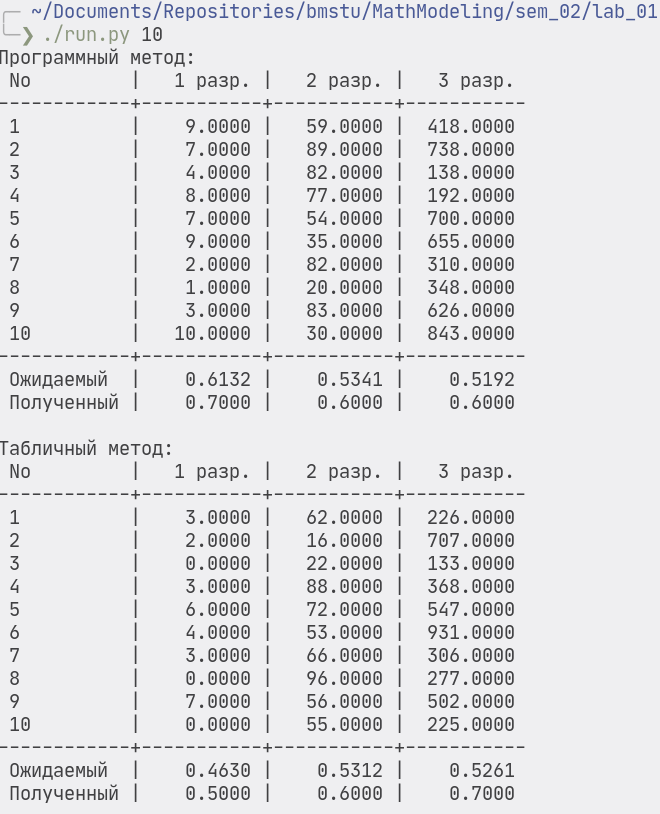
\includegraphics[width=0.8\linewidth]{images/scr01.png}
    \caption{Пример работы для 10 чисел}%
    \label{fig:scr01}
\end{figure}
\begin{figure}[htpb]
    \centering
    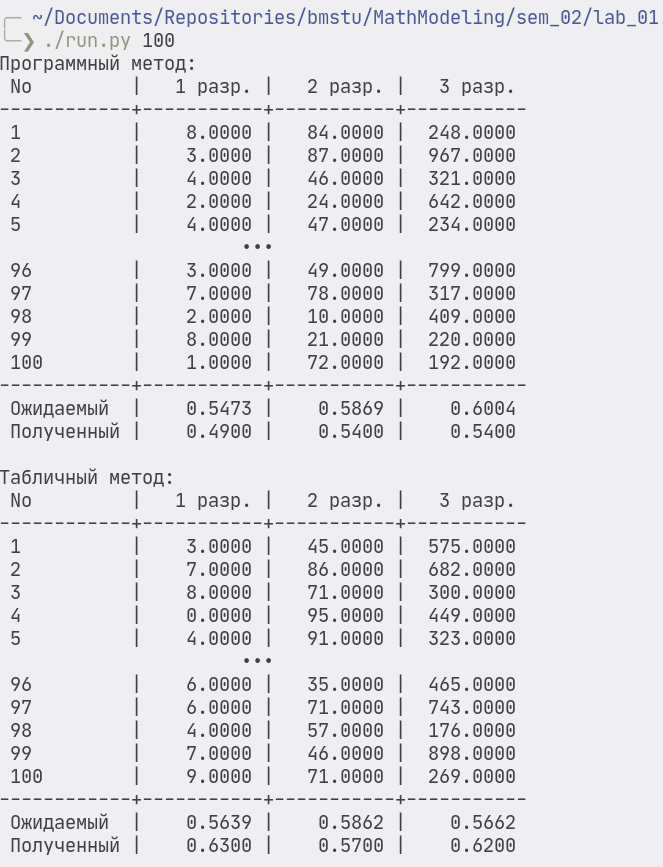
\includegraphics[width=0.8\linewidth]{images/scr02.png}
    \caption{Пример работы для 100 чисел}%
    \label{fig:scr01}
\end{figure}
\begin{figure}[htpb]
    \centering
    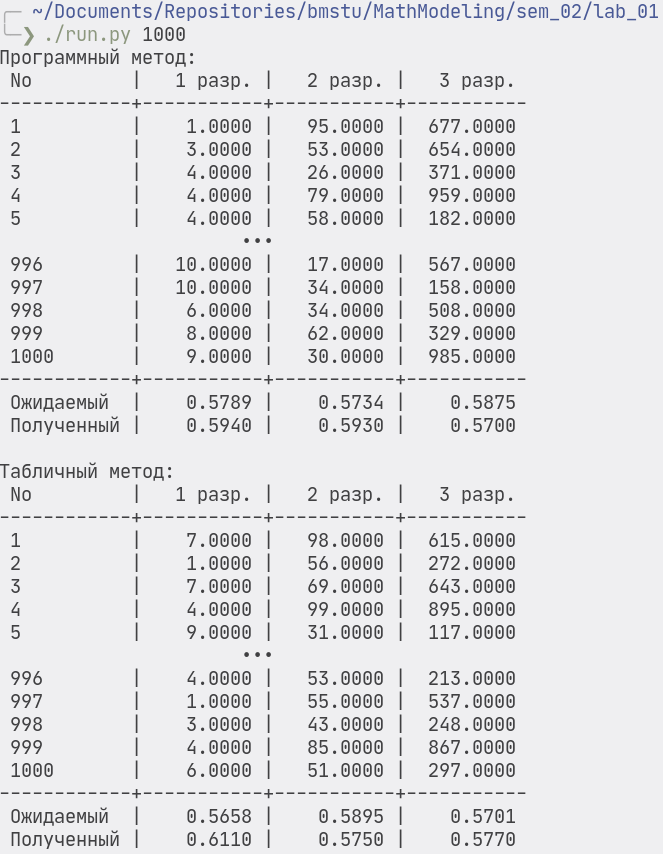
\includegraphics[width=0.8\linewidth]{images/scr03.png}
    \caption{Пример работы для 1000 чисел}%
    \label{fig:scr01}
\end{figure}

\chapter{Вывод}%
\label{cha:vyvod}

Из результатов проведённой лабораторной работы справедливо сделать вывод, что, чем больше количество генерируемых случайных чисел, тем равномернее они распределены.

Кроме того, по полученным результатам видно, что программный метод создаёт более равномерную последовательность случайных чисел, чем табличный.
